\documentclass{article}
\usepackage[utf8]{inputenc}
\usepackage{graphicx}

\title{Autonomous Agents \\ Assignment 1 \\ Group 2}
\author{Louis Smit (10678697) \\ Jerome Cremers (10470425) \\
Hubert Szostek (10656804) \\ Lex Utama (10660356)}
\date{September 2013}

\begin{document}

\maketitle

\section{Introduction}
In this assignment several single agent planning methods are implemented on a predator-prey game, as decribed in the assignment. The basic environment is an 11x11 grid (\ref{Grid}). The grid is
toroidal: the north side of the grid is attached to the south side, and the east side is attached to the west side. The predator and the prey can be anywhere on this grid, though they cannot be on the same square. The starting position of the prey is (5,5) and that of the predator (0,0).\\
Obviously, the goal for the predator is to catch the prey. This happens when the predator stands next to the prey, and moves in the direction of the prey. When the prey is captured, the episode ends, and the game is reverted to the starting position.

\begin{figure}[hb]
  \centering
  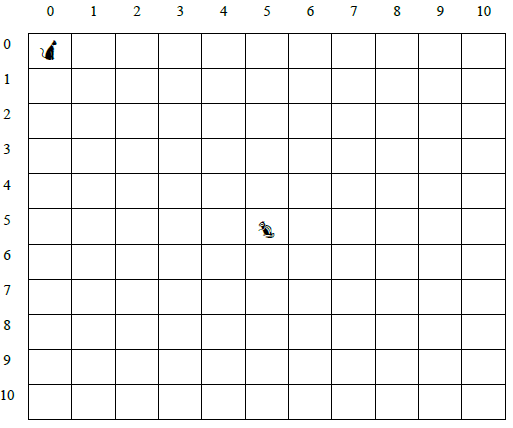
\includegraphics[width=3.3in]{Grid_world}
  \caption[Figure 1]
   {The predator-prey environment: a 11x11 toroidal grid, in the starting position. The predator is depicted by the cat, and the prey by the squirrel.}
   \label{Grid}
\end{figure}


\section{Implementation}
The game is implemented in Java. Eclipse was used as a code editor and compiler. \\
Classes\\
State space representation\\

\subsection{Policy Evalutation}
Iterative policy evaluation was implemented for the randomly moving predator. This algorithm takes a predator policy as input and produces a value for each possible state which is calculated according to the following formula: \\

\begin{math}
  V(s) = \sum_a \pi (s, a) \sum_{s'} \mathcal{P}_{ss'}^a \left[\mathcal{R}_{ss'}^a + \gamma V(s') \right]
\end{math} \\

This algorithm loops over all states until it finds that the difference between the previous value for $V(s)$ and the updated value is less than a certain threshold for all states. In the case of this specific implementation, a threshold of 0.0001 was used.

Value iteration\\
Tests\\

\section{Application Manual}
Using the built application, the results from section \ref{sec:results} can be recreated. After compilation, the application can be run using the main-method of hunt.scripts.ScriptsMenu without any arguments. This loads a textual interface, wherein commands may be invoked with optionally a set of arguments. The first word on the line should be the command, the rest of the line may contain space-separated arguments. The following commands are available:

\begin{itemize}
  \item simulator - runs a simulation using a random prey and a random predator.
  \item evaluate - runs the policy evaluator. Arguments include:
    \subitem smart - use the improved state representation.
  \item evaluate - runs the value iterator. Arguments include:
    \subitem smart - use the improved state representation.
  \item exit - terminates the program.
\end{itemize}

\section{Results}
\label{sec:results}

\subsection{Assignment 1.2}
Using the policy evaluation script, the policy for the randomly moving predator was evaluated. The values for a few of the states are listed in Table \ref{tab-poleval}. As can be seen, the states in which the predator is close to the prey receive a higher value as the predator is more likely to stumble upon the prey and receive its reward for catching it. The distance between predator and prey is equal in the second and third row, explaining why their state values are equal. In total, the algorithm required 15 sweeps to converge. \\

\begin{table}
\begin{center}
  \begin{tabular}{l | l | l}
     Predator position & Prey position & State value \\
    \hline
    5,5 & 0,0 & 0.0051 \\
    5,4 & 2,3 & 0.1812 \\
    10,0 & 2,10 & 0.1812 \\
    0,0 & 10,10 & 1,194
  \end{tabular}
  \caption{State values}
  \label{tab-poleval}
\end{center}
\end{table}

\subsection{Assignment 1.5}
In this assignment, a new internal state representation is implemented. Instead of using the old state representation wherine the absolute positions of both the predator and the prey are stored, this new representation only holds the distance between the predator and the prey, expressed as a tuple of the horizontal distance and the vertical distance. This representation is possible without violating the Markov property due to the toroidal nature of the board. \\

The new state representation has important consequences for the size of the state space. In the old representation, both the predator and the prey could be in one of $11 \times 11$ locations, amounting for a total of $11 \times 11 \times 11 \times 11 = 14641$ states. In the new representation, the distance between predator and prey can be represented as one of $11 \times 11 = 121$ states, reducing the state space by a factor $121$.

As a result, the scripts for policy evaluation and value iteration written earlier have been sped up. In the old representation, policy evaluation took 2.997 seconds, which has been improved to 1.968 seconds. A larger improvement was found for value iteration, which improved from 1.361, 2.424, 2.822 and 3.058 seconds to 0.035, 0.014, 0.039 and 0.017 seconds respectively for different values of the discount factor.

The best results in terms of time and number of iterations are observed for gamma equals 0.1. Increasing gamma factor causes increasing both factors. Changing data representation to distance based not only decrease computing time but also number of iterations. It can be observed that value iteration script performs approximately 100 times faster in comparison to the classic representation where positions of prey and predators are stored.

\section{Conclusion}

\end{document}
